\documentclass{article}
\usepackage[utf8]{inputenc}
\usepackage{listings}
\usepackage{multimedia} % to embed movies in the PDF file
\usepackage{graphicx}
\usepackage{comment}
\usepackage[english]{babel}
\usepackage{amsmath}
\usepackage{amsfonts}
\usepackage{wrapfig}
\usepackage{multirow}
\usepackage{verbatim}
\usepackage{float}
\usepackage{cancel}
\usepackage{caption}
\usepackage{subcaption}
\usepackage{/home/cade/Homework/latex-defs}
\usepackage{/home/cade/Homework/jlcode}


\title{AMATH 586 Homework 2}
\author{Cade Ballew \#2120804}
\date{April 22, 2022}

\begin{document}
	
\maketitle
	
\section{Problem 1}
To derive a 3rd order RK method, we choose to make our method explicit for ease of implementation, so by page 128 of the text, our method must have at least $r=3$ stages. We arrive at the Butcher tableau 
\[
\renewcommand\arraystretch{1.2}
\begin{array}
	{c|ccc}
	c_1 & a_{11}&a_{12}&a_{13}\\
	c_2 &a_{21} &a_{22} &a_{22}\\
	c_3 &a_{31} &a_{32} &a_{33}\\
	\hline
	1& b_1 &b_2 &b_3
\end{array}
\]
By (5.35), for consistency we need that 
\[
\sum_{j=1}^{3}a_{ij}=c_i, \quad i=1,2,3,
\]
\[
\sum_{j=1}^{3}b_j=1.
\]
By (5.37), for 2nd order accuracy we need that
\[
\sum_{j=1}^{3}b_jc_j=\frac{1}{2}.
\]
By (5.38), for 3rd order accuracy we need that
\[
\sum_{j=1}^{3}b_jc^2_j=\frac{1}{3},
\]
\[
\sum_{i=1}^{3}\sum_{j=1}^{3}b_ia_{ij}c_j=\frac{1}{6}.
\]
Since we want our method to be explicit, we set all $a_{ij}$ on or above the diagonal to zero which leaves us with the Butcher tableau
\[
\renewcommand\arraystretch{1.2}
\begin{array}
	{c|ccc}
	0 & 0&0&0\\
	c_2 &c_2 &0 &0\\
	c_3 &a_{31} &a_{32} &0\\
	\hline
	1& b_1 &b_2 &b_3
\end{array}
\]
as our first condition requires that $c_1=0$ and $a_{21}=c_2$ after we impose this. Now, in order to obtain a simple method, we set $a_{31}=b_2=0$, so our tableau becomes
\[
\renewcommand\arraystretch{1.2}
\begin{array}
	{c|ccc}
	0 & 0&0&0\\
	c_2 &c_2 &0 &0\\
	c_3 &0 &c_3 &0\\
	\hline
	1& b_1 &0 &b_3
\end{array}
\]
and the constraints that we have not already imposed become
\begin{align*}
	b_1+b_3&=1\\
	b_3c_3&=\frac{1}{2}\\
	b_3c_3^2&=\frac{1}{3}\\
	b_3c_2c_3&=\frac{1}{6}.
\end{align*}
Combining the 2nd and 3rd equations allows us to find that $c_3=\frac{2}{3}$ which then gives that $b_3=\frac{3}{4}$. Using the 1st and 4th equations, we then find that $b_1=\frac{1}{4}$ and $c_2=\frac{1}{3}$. Thus, our Butcher tableau is
\[
\renewcommand\arraystretch{1.2}
\begin{array}
	{c|ccc}
	0 & 0&0&0\\
	1/3 &1/3 &0 &0\\
	2/3 &0 &2/3 &0\\
	\hline
	1& 1/4 &0 &3/4
\end{array}
\]
Now, we use the general form for RK methods (5.34) to convert our tableau into the following scheme:
\begin{align*}
	&y_1=u^n\\
	&y_2=u^n+\frac{k}{3}f(y_1,t_n)\\
	&y_3=u^n+\frac{2k}{3}f(y_n,t_n+k/3)\\
	&u^{n+1}=u^n+k\left(\frac{1}{4}f(y_1,t_n)+\frac{3}{4}f(y_3,t_n+2k/3)\right) 
\end{align*}
for a problem $u'(t)=f(u(t),t)$. Note that this is Heun's 3rd order method. \\ 
Using Julia, we test this method on the problem $$ v'''(t) + v'(t) v(t) - \frac{\beta_1 + \beta_2 + \beta_3}{3} v'(t) =0, $$

where $\beta_1 < \beta_2 < \beta_3$ with initial conditions
$$
v(0) = \beta_3, \\
v'(0) = 0,\\
v''(0) = -\frac{(\beta_3 - \beta_1)(\beta_3-\beta_2)}{6}.$$ We turn it into a system
$$
u_1'(t) =  v'(t) = u_2(t),\\
u_2'(t) = v''(t) = u_3(t),\\
u_3''(t) = \frac{\beta_1 + \beta_2 + \beta_3}{3} u_2(t) -  u_2(t)u_1(t)
$$
and set $c = \frac{\beta_1 + \beta_2 + \beta_3}{3}$
$$
f(u) = \begin{bmatrix} u_2 \\ u_3 \\ u_2(c - u_1)\end{bmatrix}.
$$
Solving this problem for various stepsizes, we compute the error at each by comparing to the known solution of this problem. Plotting the error for each stepsize $k$ along with a reference line $g(k)=k^3$ on a log-log scale, we observe the following plot. \\
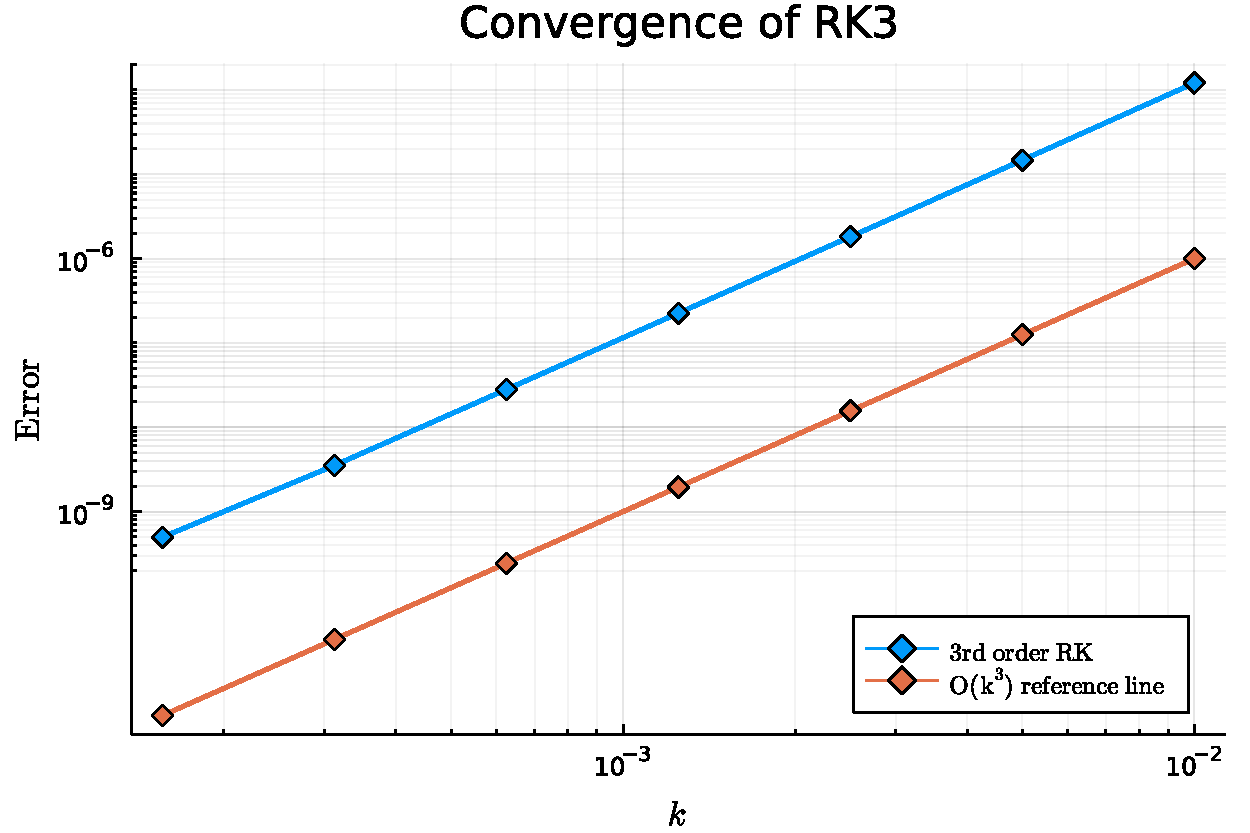
\includegraphics[scale=0.5]{p1.pdf}\\
These lines appear to be parallel meaning that our method appears to be third order as anticipated. We also print a table of error values and the error reduction ratio $$\frac{\text{Error with time step } 2k}{\text{Error with time step } k}.$$\\
\begin{verbatim}
k        | error      | error reduction   
0.010000 | 1.2102e-04 |       
0.005000 | 1.4730e-05 |      8.2161  
0.002500 | 1.8163e-06 |      8.1097  
0.001250 | 2.2547e-07 |      8.0556  
0.000625 | 2.8075e-08 |      8.0311  
0.000313 | 3.5287e-09 |      7.9562  
0.000156 | 4.9731e-10 |      7.0956
\end{verbatim}
For an $r$th-order method we should see this be approximately $2^r$, so this suggests that our method is third order as most of our values are approximately 8. \\
See Appenix A for the code used in this problem.

\section{Problem 2}
Note that a general LMM has form 
\[
\sum_{j=0}^r\alpha_ju^{n+j}=k\sum_{j=0}^r\beta_jf(u^{n+j},t_{n+j})
\]
and that (5.48) gives that such a method is consistent if
\[
\sum_{j=0}^r\alpha_j=0,
\]
\[
\sum_{j=0}^rj\alpha_j=\sum_{j=0}^r\beta_j.
\]
\subsection{Part a}
The LMM 
\[U^{n+3} = U^{n+1} + 2kf(U^n)\]
corresponds to $r=3$, $\alpha_3=1$, $\alpha_2=0$, $\alpha_1=-1$, $\alpha_0=0$, $\beta_3=\beta_2=\beta_1=0$, $\beta_0=2$. Thus, 
\[
\sum_{j=0}^r\alpha_j=0,
\]
\[
\sum_{j=0}^rj\alpha_j=3-1=2=\sum_{j=0}^r\beta_j,
\]
so it is consistent. It has characteristic polynomial
\[
\rho(\zeta)=\zeta^3-\zeta=\zeta(\zeta+1)(\zeta-1)
\]
which has roots $\zeta=0,\pm1$ which satisfy the root condition, so it is also zero-stable. Thus, the method is convergent. 

\subsection{Part b}
The LMM
\[
U^{n+2} = \half U^{n+1} + \half U^{n} + 2kf(U^{n+1})
\]
corresponds to $r=2$, $\alpha_2=1$, $\alpha_1=-\half$, $\alpha_0=-\half$, $\beta_2=\beta_0=0$, $\beta_1=2$, so
\[
\sum_{j=0}^rj\alpha_j=2-\frac{1}{2}=\frac{3}{2}\neq2=\sum_{j=0}^r\beta_j,
\]
so it is not consistent and therefore not convergent. It has characeristic polynomial
\[
\rho(\zeta)=\zeta^2-\half\zeta-\half=(\zeta+\half)(\zeta-1)
\]
which has roots $-\half,1$ meaning that it is zero-stable.

\subsection{Part c}
The LMM 
\[
U^{n+1} = U^n
\]
corresponds to $r=1$, $\alpha_1=1$, $\alpha_0=-1$, $\beta_1=\beta_0=0$, so
\[
\sum_{j=0}^rj\alpha_j=1\neq0=\sum_{j=0}^r\beta_j,
\]
so it is not consistent and therefore not convergent. It has characteristic polynomial
\[
\rho(\zeta)=\zeta-1
\]
which has root $\zeta=1$, so it is zero-stable.

\subsection{Part d}
The LMM
\[
U^{n+4} = U^{n} + \frac 4 3 k(f(U^{n+3})+f(U^{n+2})+f(U^{n+1}))
\]
corresponds to $r=4$, $\alpha_4=1$, $\alpha_3,\alpha_2,\alpha_1=0$, $\alpha_0=-1$, $\beta_4=0$, $\beta_3=\beta_2=\beta_1=\frac{4}{3}$, $\beta_0=0$, so 
\[
\sum_{j=0}^r\alpha_j=0,
\]
\[
\sum_{j=0}^rj\alpha_j=4=3\cdot\frac{4}{3}=\sum_{j=0}^r\beta_j,
\]
meaning that it is consistent. It has characteristic polynomial
\[
\rho(\zeta)=\zeta^4-1
\]
which has roots $\zeta=\pm1,\pm i$ which all have magnitude 1 but are not repeated, so the root condition is satisfied. Thus, it is zero-stable meaning that it is also convergent. 

\subsection{Part e}
The LMM 
\[
U^{n+3} = -U^{n+2} + U^{n+1} +U^{n}+2k(f(U^{n+2})+f(U^{n+1}))
\]
corresponds to $r=3$, $\alpha_3=\alpha_2=1$, $\alpha_1=\alpha_0=-1$, $\beta_3=\beta_0=0$, $\beta_2=\beta_1=2$, so
\[
\sum_{j=0}^r\alpha_j=0,
\]
\[
\sum_{j=0}^rj\alpha_j=3+2-1=4=\sum_{j=0}^r\beta_j,
\]
so it is consistent. However, it has characteristic polynomial 
\[
\rho(\zeta)=\zeta^3+\zeta^2-\zeta-1=(\zeta-1)(\zeta+1)^2
\]
which has roots $\zeta=\pm1$. While these both have magnitude 1, the $\zeta=-1$ root is repeated, so the root condition is not satisfied and it is not zero-stable and therefore not convergent. 

\section{Problem 3}
\subsection{Part a}
Consider the recursion
\[
U^{n+2} = U^{n+1} + U^n.
\]
To find a general solution, we make an ansatz $U^n=\zeta^n$ so that we can consider the charcteristic polynomial
\[
\rho(\zeta)=\zeta^2-\zeta-1=0.
\]
The roots of this polynomial are given by
\[
\zeta_{1,2}=\frac{1\pm\sqrt{5}}{2},
\]
so our general solution is given by
\[
U^n=c_1\left(\frac{1-\sqrt{5}}{2}\right)^n+c_2\left(\frac{1+\sqrt{5}}{2}\right)^n.
\]

\subsection{Part b}
If we take starting values $U^0=1$, $U^1=1$, we can plug these into our general solution and determine $c_1,c_2$ by solving the linear system
\begin{align*}
	\begin{cases}
		c_1+c_2=1\\
		c_1\frac{1-\sqrt{5}}{2}+c_2\frac{1+\sqrt{5}}{2}=1.
	\end{cases}
\end{align*}
Substituting the first equation into the second, ,
\[
c_1\frac{1-\sqrt{5}}{2}+(1-c_1)\frac{1+\sqrt{5}}{2}=1,
\]
so
\[
c_1=\frac{1-\frac{1+\sqrt{5}}{2}}{\frac{1-\sqrt{5}}{2}-\frac{1+\sqrt{5}}{2}}=\frac{1}{-\sqrt{5}}\frac{1-\sqrt{5}}{2}=\frac{5-\sqrt{5}}{10},
\]
and
\[
c_2=1-\frac{5-\sqrt{5}}{10}=\frac{5+\sqrt{5}}{10}.
\]
Thus, 
\[
U^n=\frac{5-\sqrt{5}}{10}\left(\frac{1-\sqrt{5}}{2}\right)^n+\frac{5+\sqrt{5}}{10}\left(\frac{1+\sqrt{5}}{2}\right)^n,
\]
so we can use Wolfram-Alpha to plug $n=30$ into this formula and conclude that
\[
U^{30}=1346269.
\]

\subsection{Part c}
Now, note that because $\left|\frac{1+\sqrt{5}}{2}\right|>1$, $\left|\frac{1-\sqrt{5}}{2}\right|<1$,
\begin{align*}
\lim_{n\to\infty}\frac{u^n}{u^{n-1}}=\frac{\frac{5-\sqrt{5}}{10}\cancelto{0}{\left(\frac{1-\sqrt{5}}{2}\right)^n}+\frac{5+\sqrt{5}}{10}\left(\frac{1+\sqrt{5}}{2}\right)^n}{\frac{5-\sqrt{5}}{10}\cancelto{0}{\left(\frac{1-\sqrt{5}}{2}\right)^{n-1}}+\frac{5+\sqrt{5}}{10}\left(\frac{1+\sqrt{5}}{2}\right)^{n-1}}=\frac{1+\sqrt{5}}{2}=\phi.
\end{align*}

\section{Problem 4}
Consider the difference equation
\begin{align*}
	U^{n+1} &+ U^{n-1} = 2x U^n, \quad n \geq 0,\\
	U^0 &= 1, \quad U^{-1} = 0
\end{align*}
where $-1 \leq x \leq 1$.

\subsection{Part a}
Since $-1 \leq x \leq 1$ and the cosine function takes on all values between $-1$ and $1$, we know that $x=\cos\theta$ for some $\theta\in\real$. By definition,
\[
\cos\theta=\frac{e^{i\theta}+e^{-i\theta}}{2},
\]
so our difference equation becomes
\begin{align*}
	U^{n+1} &+ U^{n-1} = (e^{i \theta} + e^{- i \theta}) U^n, \quad n \geq 0,\\
	U^0 &= 1, \quad U^{-1} = 0, \quad \theta \in \mathbb R.
\end{align*}

\subsection{Part b}
If we define $V^n = U^n - e^{i \theta} U^{n-1}$, we can use our recurrence to find that
\begin{align*}
V^n &= U^n - e^{i \theta} U^{n-1}=U^n -e^{i \theta}(-U^{n+1}+(e^{i \theta} + e^{- i \theta}) U^n)\\&=
e^{i\theta}U^{n+1}-e^{2i\theta}U^n=e^{i\theta}(U^{n+1}+e^{i\theta}U^n)=e^{i\theta}V^{n+1},
\end{align*}
so $V^{n+1}=e^{-i\theta}V^n$. Note that our initial conditions give that $V^0=1$, so we now have the recurrence 
\begin{align*}
	V^{n+1}&=e^{-i\theta}V^n, \quad n \geq 0,\\
	V^0 &= 1, \quad \theta \in \mathbb R.
\end{align*}
Now, this recurrence has characteristic polynomial
\[
\rho(\zeta)=\zeta-e^{-i\theta}
\]
which has root $\zeta=e^{-i\theta}$, so we have general solution
\[
V^n=c(e^{-i\theta})^n.
\]
Plugging in $n=0$, we find that $c=1$, so 
\[
V^n=e^{-in\theta}.
\] 

\subsection{Part c}
Having solved for $V^n$, we now have the nonlinear recurrence relation 
\begin{align*}
	U^{n}&=e^{i\theta}U^{n-1}+e^{-in\theta}, \quad n \geq 1,\\
	U^0 &= 1, \quad \theta \in \mathbb R.
\end{align*}
To solve this, note that a general nonlinear recurrence $u^n=\alpha u^{n-1}+h_n$ has solution
\begin{align*}
u^1&=\alpha u^0+h_1\\
u^2&=\alpha^2u^0+\alpha h_1+h_2\\
u^3&= \alpha^3u^0+\alpha^2 h_1+\alpha h_2+h_3\\
&\vdots\\
u^n&=\alpha^n u^0+\sum_{j=1}^{n}\alpha^{n-j}h_{j}.
\end{align*}
Here, we have $u^0=U^0=1$, $\alpha=e^{i\theta}$, $h_n=e^{-in\theta}$, so we have that for $n\geq1$, 
\begin{align*}
U^n=e^{in\theta}+\sum_{j=1}^{n}e^{i(n-j)\theta}e^{-ij\theta}=e^{in\theta}+\sum_{j=1}^{n}e^{i(n-2j)\theta}=\sum_{j=0}^{n}e^{i(n-2j)\theta}.
\end{align*}
If $n$ is odd,
\begin{align*}
U^n=\sum_{j=0}^{(n-1)/2}e^{i(n-2j)\theta}+\sum_{j=(n+1)/2}^{n}e^{i(n-2j)\theta}.
\end{align*}
Making the change of index $j\to n-j$ in the second sum,
\begin{align*}
	U^n&=\sum_{j=0}^{(n-1)/2}e^{i(n-2j)\theta}+\sum_{j=(n-1)/2}^{0}e^{i(n-2(n-j))\theta}=\sum_{j=0}^{(n-1)/2}(e^{i(n-2j)\theta}+e^{-i(n-2j)\theta})\\&=
	2\sum_{j=0}^{(n-1)/2}\cos(n-2j)\theta. 
\end{align*}
If we again reindex, $j\to \frac{n-1-2j}{2}$,
\[
U^n=2\sum_{j=0}^{(n-1)/2}\cos(2j+1)\theta.
\]
If $n$ is even, 
\begin{align*}
	U^n=\sum_{j=0}^{n/2-1}e^{i(n-2j)\theta}+e^{i(n-n)\theta}+\sum_{j=n/2+1}^{n}e^{i(n-2j)\theta}.
\end{align*}
Reindexing $j\to n-j$ in the second sum,
\begin{align*}
	U^n&=1+\sum_{j=0}^{n/2-1}e^{i(n-2j)\theta}+\sum_{j=n/2-1}^{0}e^{i(n-2(n-j))\theta}=1+\sum_{j=0}^{n/2-1}(e^{i(n-2j)\theta}+e^{-i(n-2j)\theta})\\&=
	1+2\sum_{j=0}^{n/2-1}\cos(n-2j)\theta. 
\end{align*}
Again reindexing $j\to n/2-j$,
\[
U^n=1+2\sum_{j=1}^{n/2}\cos2j\theta.
\]
To find the $x$ such that $U^n$ is maximized, we again need to consider the even and odd cases separately. In the case where $n$ is odd, each term in the series is of the form $\cos k\theta$ where $k$ is odd. The cosine function has maximum value 1 which it obtains at arguments of the form $2k\pi$ where $k\in\mathbb{Z}$. In the case where $n$ is odd, if we have  that $(2j+1)\theta=2k\pi$ for $j=0,\ldots,(n-1)/2$, then $U^n$ must be maximized. In order for this to hold at $j=0$, we need that $\theta=2k\pi$ for $k\in \mathbb{Z}$. If $\theta$ has this form, then clearly $(2j+1)\theta=2k'\pi$ for some $k'\in\mathbb{Z}$, so each term of the sum is maximized. Thus, $U^n$ is maximized at $\theta=2k\pi$ for $k\in \mathbb{Z}$. This gives that $x=\cos2k\pi=1$, so $U^n$ is maximized at $x=1$.\\
If $n$ is even, we have  that if $2j\theta=2k\pi$ for $j=1,\ldots,n/2$, then $U^n$ must be maximized since its individual components are maximized. In order for this to hold at $j=1$, we need that $\theta=k\pi$ where $k\in\mathbb{Z}$. If $\theta$ has this form,  then clearly $2j\theta=2k'\pi$ for some $k'\in\mathbb{Z}$, so each term of the sum is maximized. Thus, $U^n$ is maximized at $\theta=k\pi$ for $k\in Z$. This gives that $x=\cos k\pi=\pm1$, so $U^n$ is maximized at $x=\pm1$.

\section{Problem 5}
Consider the RK4 method of example 5.13 in the text applied to the problem $u'(t) = \lambda u(t)$. We find that if $z=k\lambda$,
\begin{align*}
y_1&=u^n\\
y_2&=u^n+\frac{1}{2}k\lambda y_1=\left(1+\frac{z}{2}\right)u^n\\
y_3&=u^n+\frac{1}{2}k\lambda y_2=\left(1+\frac{z}{2}+\frac{z^2}{4}\right)u^n\\
y_4&=u^n+k\lambda y_3=\left(1+z+\frac{z^2}{2}+\frac{z^3}{4}\right)u^n\\
u^{n+1}&=u^n+\frac{k\lambda}{6}\left(y_1+2y_2+2y_3+y_4\right)=\left(1+\frac{z}{6}\left(6+3z+z^2+\frac{z^3}{4}\right)\right)u^n\\&=
\left(1+z+\frac{z^2}{2}+\frac{z^3}{6}+\frac{z^4}{24}\right)u^n.
\end{align*}
This implies that 
\[
R(z)=1+z+\frac{z^2}{2!}+\frac{z^3}{3!}+\frac{z^4}{4!}
\]
which clearly matches the power series of $e^z$ through the fourth order.

\section{Problem 6}
Applying the simplification of TR-BDF2 given in (8.6) to the problem $u'(t) = \lambda u(t)$, we first have that 
\[
u^*=u^n+\frac{k}{4}(\lambda u^n+\lambda u^*),
\]
so we can find that
\[
u^*=\frac{4+z}{4-z}
\]
where $z=k\lambda$. We then have that
\[
u^{n+1}=\frac{1}{3}(4u^*-u^n+k\lambda u^{n+1}).
\]
Using our value of $u^*$, 
\begin{align*}
3u^{n+1}=\left(4\frac{4+z}{4-z}-1\right)u^n+zu^{n+1},
\end{align*}
so 
\[
(3-z)u^{n+1}=\frac{12+5z}{4-z}u^n,
\]
and 
\[
u^{n+1}=\frac{12+5z}{(3-z)(4-z)}u^n,
\]
so we have 
\[
R(z)=\frac{12+5z}{(3-z)(4-z)}.
\]
Now, we expand
\[
\frac{1}{3-z}=\frac{1}{3}\frac{1}{1-\frac{z}{3}}=\frac{1}{3}\sum_{j=0}^{\infty}\left(\frac{z}{3}\right)^j=\sum_{j=0}^{\infty}\frac{z^j}{3^{j+1}}.
\]
Similarly, 
\[
\frac{1}{4-z}=\sum_{j=0}^{\infty}\frac{z^j}{4^{j+1}}.
\]
Now, using the Cauchy product,
\begin{align*}
\frac{1}{(3-z)(4-z)}=\sum_{j=0}^{\infty}\frac{z^j}{3^{j+1}}\sum_{k=0}^{\infty}\frac{z^k}{4^{k+1}}=\sum_{j=0}^{\infty}\sum_{\ell=0}^j\frac{z^\ell}{3^{\ell+1}}\frac{z^{j-\ell}}{4^{j-\ell+1}}=\sum_{j=0}^{\infty}\sum_{\ell=0}^j\frac{z^j}{3^{\ell+1}4^{j-\ell+1}}.
\end{align*}
Thus,
\begin{align*}
R(z)&=(12+5z)\sum_{j=0}^{\infty}\sum_{\ell=0}^j\frac{z^j}{3^{\ell+1}4^{j-\ell+1}}=\sum_{j=0}^{\infty}\sum_{\ell=0}^j\left(\frac{12z^j}{3^{\ell+1}4^{j-\ell+1}}+\frac{5z^{j+1}}{3^{\ell+1}4^{j-\ell+1}}\right)\\&=
1+\left(\left(\frac{z}{3}+\frac{z}{4}\right)+\frac{5z}{12}\right)+\left(\left(\frac{z^2}{16}+\frac{z^2}{12}+\frac{z^2}{9}\right)+\left(\frac{5z^2}{36}+\frac{5z^2}{48}\right)\right)+\ldots\\&=
1+z+\frac{z^2}{2}+\ldots
\end{align*}
which clearly matches the power series of $e^z$ through the second order.

\section{Problem 7}
Consider the time-dependent matrices
\begin{align*}
	T_N(t) &= \begin{bmatrix}
		b_1(t) & a_1(t)\\
		a_1(t) & b_{2}(t) & a_{2}(t)\\
		& a_{2}(t) & b_{3}(t) & \ddots\\
		&& \ddots & \ddots & a_{N-1}(t) \\
		&&& a_{N-1}(t) & b_N(t)
	\end{bmatrix},\\
	S_N(t) &= \begin{bmatrix}
		0 & a_1(t)\\
		-a_1(t) & 0 & a_{2}(t)\\
		& -a_{2}(t) & 0 & \ddots\\
		&& \ddots & \ddots & a_{N-1}(t) \\
		&&& -a_{N-1}(t) & 0.
	\end{bmatrix}
\end{align*}
With initial conditions $b_j(0) = 0$, $j = 1,2,\ldots,N$, $a_j(0) = 1/2, j = 1,2,\ldots,N-1$ and $N = 6$. In Julia, we use RK4 to solve 
\begin{align*}
	T_N'(t) = S_N(t) T_N(t) - T_N(t)S_N(t),
\end{align*}
to $t = 100$ and plot the $a_j(t),b_j(t)$. \\
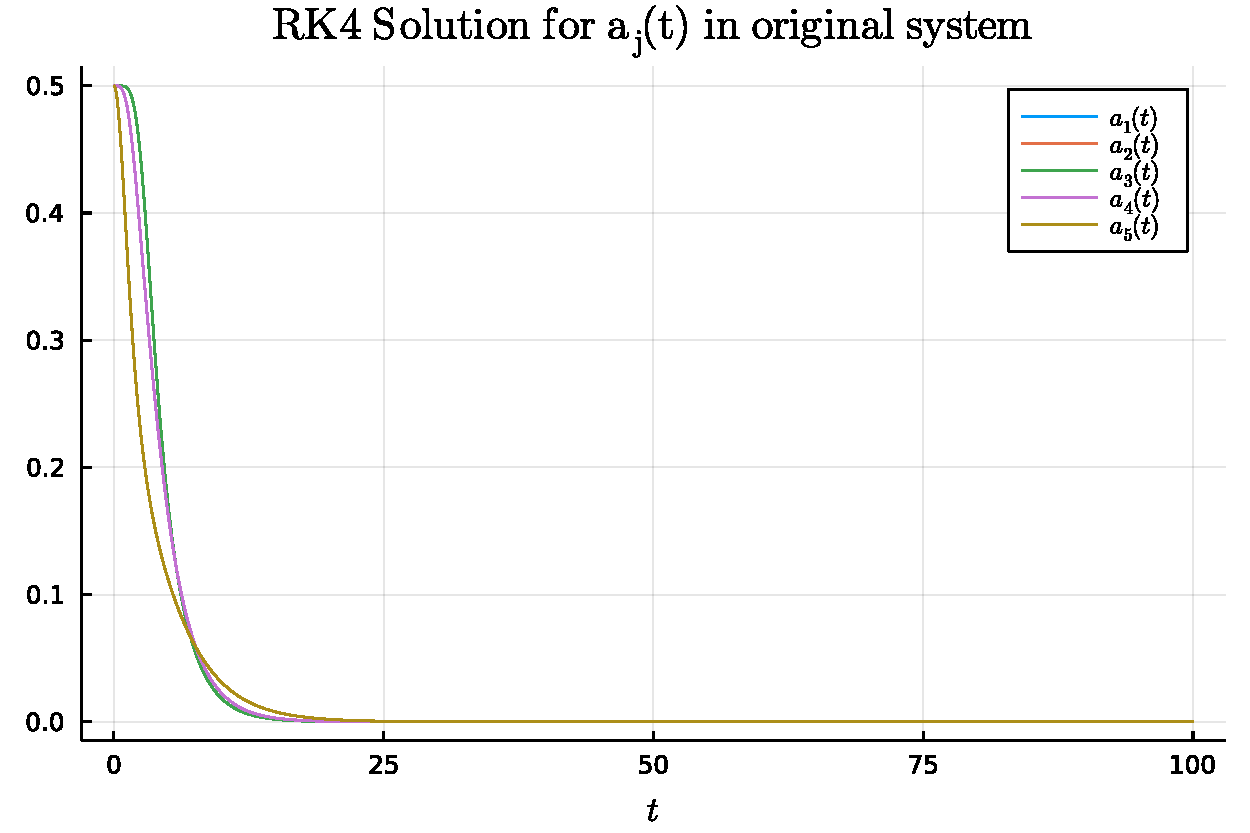
\includegraphics[scale=0.5]{p7ii.pdf}\\
\\
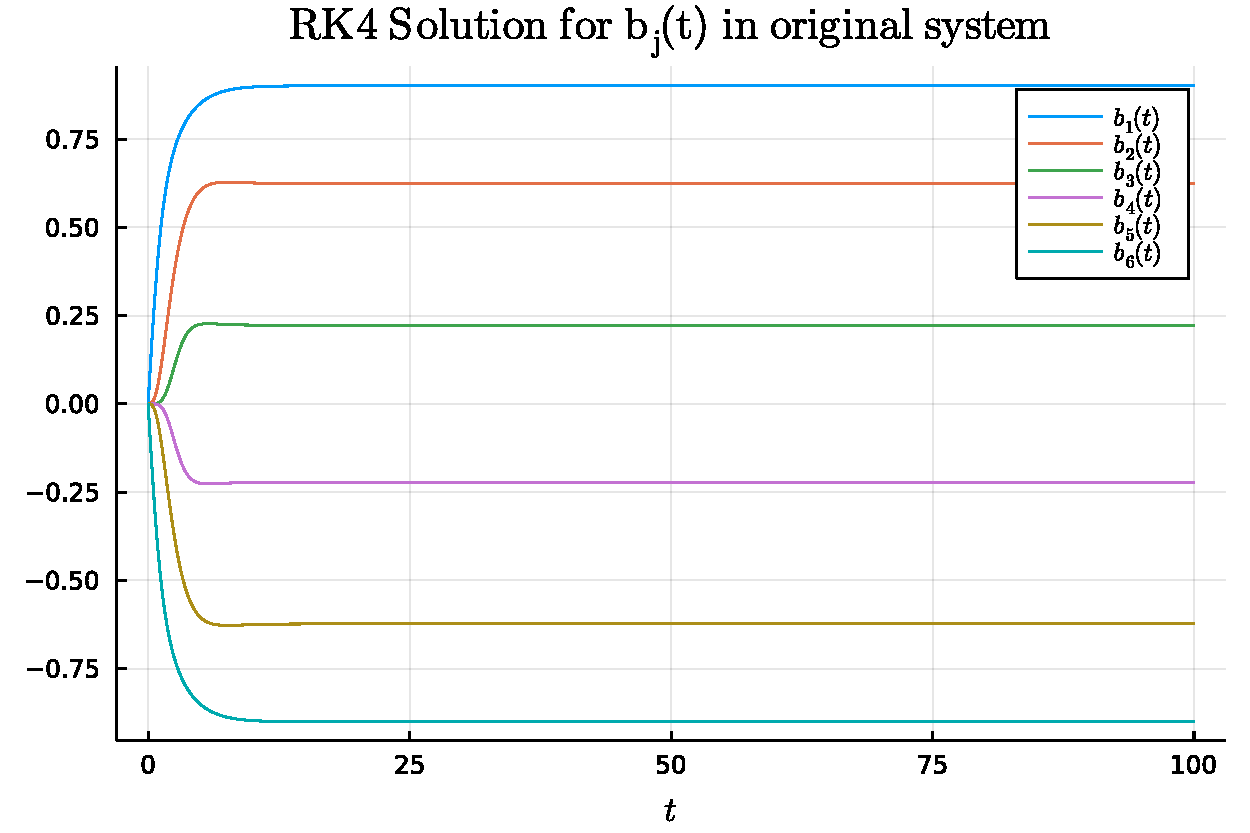
\includegraphics[scale=0.5]{p7i.pdf}\\
It appears that the off-diagonal entries of $T_N(t)$ tend to zero and the diagonal entries tend to the eigenvalues of $T_N(0)$. This is because the matrices constitute a Lax pair which implies that the eigenvalues of $T_N(t)$ are independent of $t$, so if the off-diagonal entries tend to zero, the diagonal entries must tend to the eigenvalues.\\
Now, consider $b_j(0) = -2$ and $a_j(0) = 1$, $j = 1,2,\ldots,N$ and $N = 12$. Again using RK4 in Julia, we obtain the following plots.\\
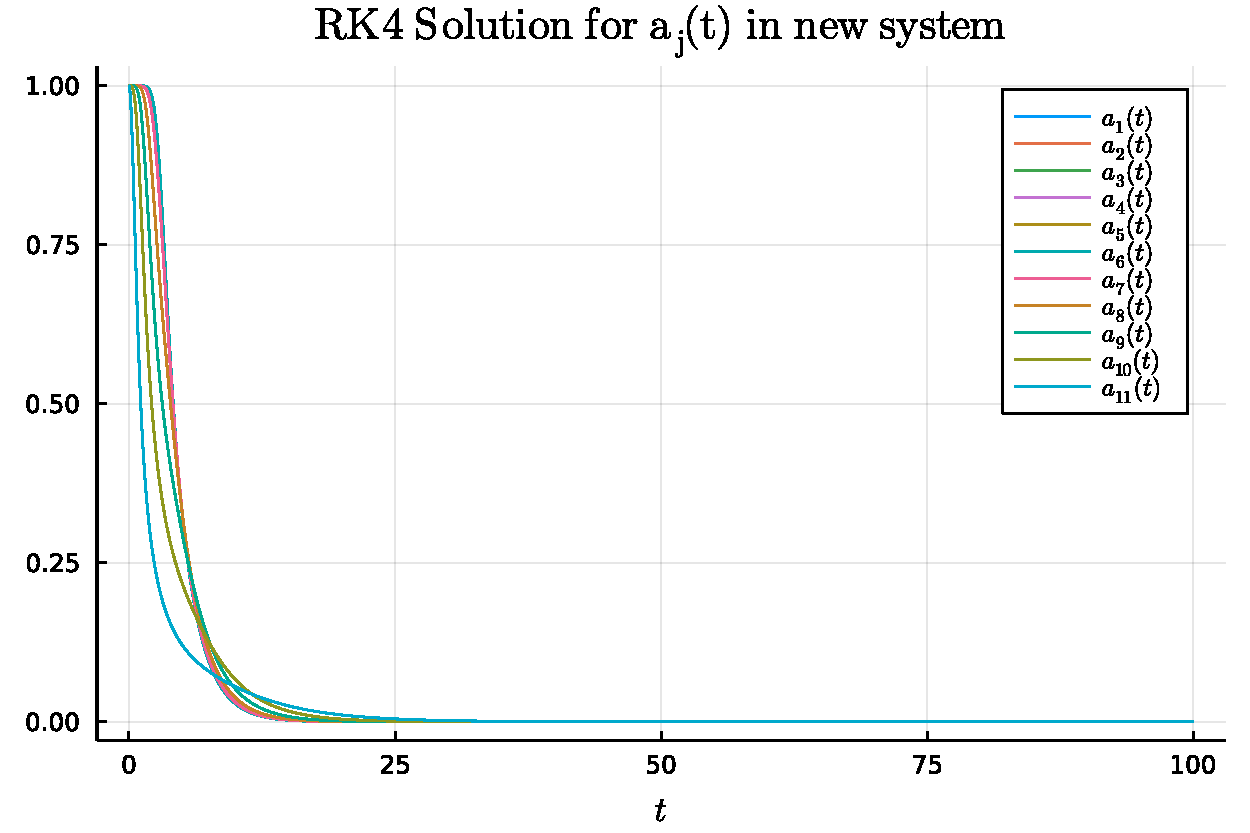
\includegraphics[scale=0.5]{p7iv.pdf}\\
\\
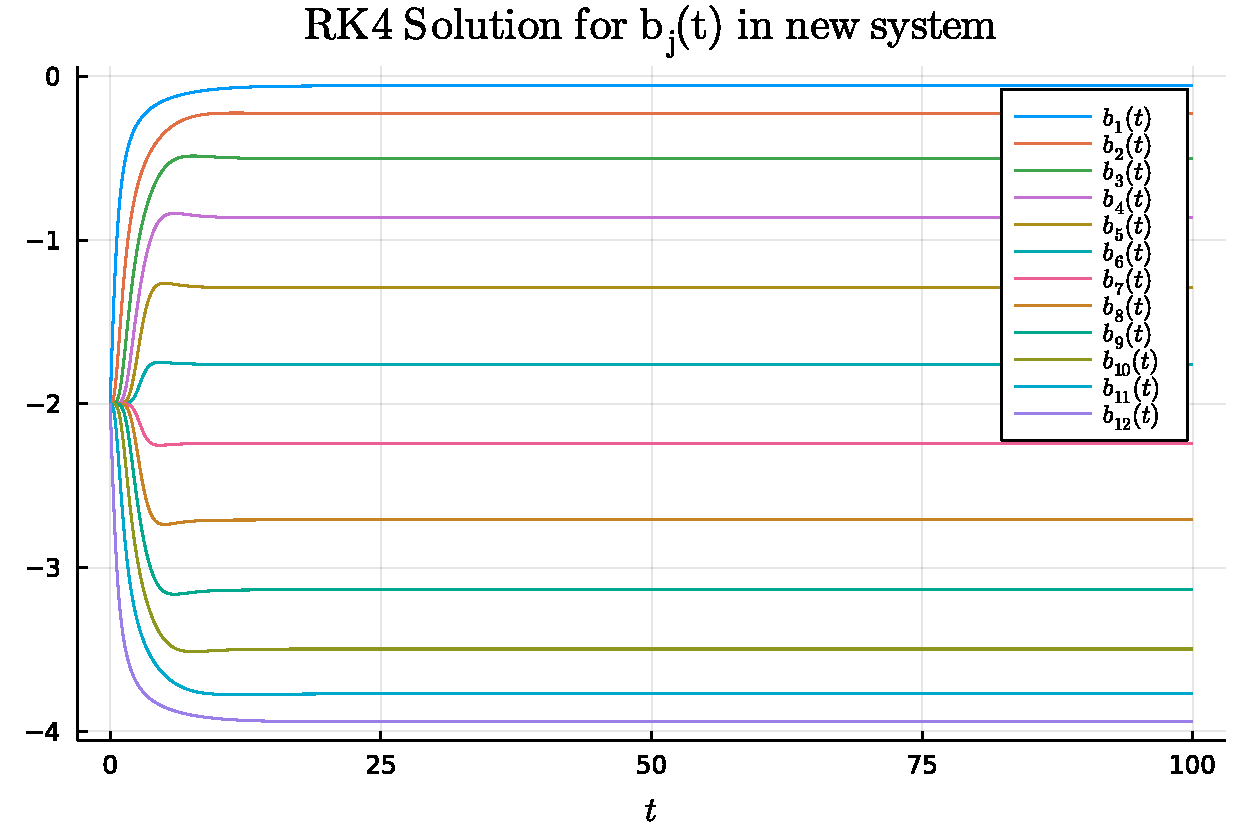
\includegraphics[scale=0.5]{p7iii.pdf}\\
Again, it appears that the off-diagonal entries of $T_N(t)$ tend to zero and the diagonal entries tend to the eigenvalues of $T_N(0)$.\\
See Appendix A for the Julia code used to solve this problem.

\section{Appendix A}
The following is the code used for problem 1.
\jlinputlisting{Problem1.jl}
The following is the code used from problem 7. 
\jlinputlisting{Problem7.jl}

\end{document}
